\documentclass[12pt,letterpaper]{article}
\usepackage{fullpage}
\usepackage[top=2cm, bottom=4.5cm, left=2.5cm, right=2.5cm]{geometry}
\usepackage{amsmath,amsthm,amsfonts,amssymb,amscd}
\usepackage{lastpage}
\usepackage{enumerate}
\usepackage{fancyhdr}
\usepackage{hyperref}
\usepackage{pythontex}
\usepackage[siunitx]{circuitikz}
\usepackage{color} %red, green, blue, yellow, cyan, magenta, black, white
\usepackage[inline]{enumitem}
\usepackage{booktabs}
\usepackage{relsize}
\usepackage{calculator}
\usepackage{siunitx}
\usepackage{appendix}
\usepackage{listings}
\usepackage{steinmetz}

\setlength{\parindent}{0.0in}
\setlength{\parskip}{0.05in}

% Edit these as appropriate
\definecolor{mygreen}{RGB}{28,172,0} % color values Red, Green, Blue
\definecolor{mylilas}{RGB}{170,55,241}

\newcommand\course{MCEN 5228-004}
\newcommand\project{3}                  % <-- homework number
\newcommand\NetIDa{Coovi Meha}           % <-- NetID of person #1
\newcommand\NetIDb{MEid:481-473}           % <-- NetID of person #2 (Comment this line out for problem sets)

\pagestyle{fancyplain}
\headheight 35pt
\lhead{\NetIDa}
\lhead{\NetIDa\\\NetIDb}                 % <-- Comment this line out for problem sets (make sure you are person #1)
\chead{\textbf{\Large Project \project}}
\rhead{\course \\ \today}
\lfoot{}
\cfoot{}
\rfoot{\small\thepage}
\headsep 1.5em
\begin{document}
\begin{pycode}

\end{pycode}
\section*{Abstract}
In Engineering, most designs revolve around using analog  and digital devices. Thus, the conversion of data from one type to 
another becomes necessary to achieve a desired goal in building a project. Data which will be refereed to as a signal during
in this report can be discrete or analog. Analog signals are continued while discrete signal are discretized data points sampled
at a specific frequency (period) by computerize device. \\
Let assume that we have e system consist of a MyRio  and a motor; and we wish to record the speed of the 
while running a feedback loop. To achieve this, the MyRio must record the voltage output from the motor, take it through the 
feedback loop then output a new a corrected signal to make the motor run at a constant speed. However, it is important to note that computer runs
in discrete time while the motor runs in continues time leading to the necessity to convert the signal between analog (continue time signal ) and digital(discrete time signal).\\
The conversion process is themed signal reconstruction. This report will center on how reconstruction can be performed, the 
problem that can arise during signal processing with examples and some solution to help be a master at reconstructing signal. To 
achieve the above we must assume the following:
\begin{itemize}
    \item The system must be causal: We can not see the future in another word the system response time start at t=0s. 
    \item Linear time invariant system: The system is linear and time independent.
\end{itemize}
\section*{What is signal reconstruction?}
Sampling of signals consist of the snapshot the continues time signal at a constant
time intervals. The process leads generality to collection data points of different amplitudes
with a certain period or frequency called the sampling period. The reconstruction of this 
signal despite the opposite of the previous process with a continuous signal 
similar to the original signal sampled. But first what does sampling look like from Engineering
prospective?
\subsection*{Sampling}
Consider the following signal in continue time domain. 
\begin{equation}
    f(t)=sin(2\pi t) +0.2cos(12\pi t)
\end{equation}
If one wants to plot this function in Matlab for example, it is necessary to generate discrete points
by defining the small enough time interval that can give a good resolution to the plot. This
is a discrimination of the continuos time signal function. The similar method is used when sampling a signal.
However, instead we define an impulse function 
\begin{equation}
    f_i(t)=T\sum_{k=-\infty}^{\infty} \delta(x-kT)
\end{equation}
to slash the continuous signal into discrete data points
the impulse signal must have a high of exactly one to allow avery point generated to have the 
same amplitudes as in the continuous function. The following illustration give a better view of the 
process
\begin{figure}[h]
    \centering
        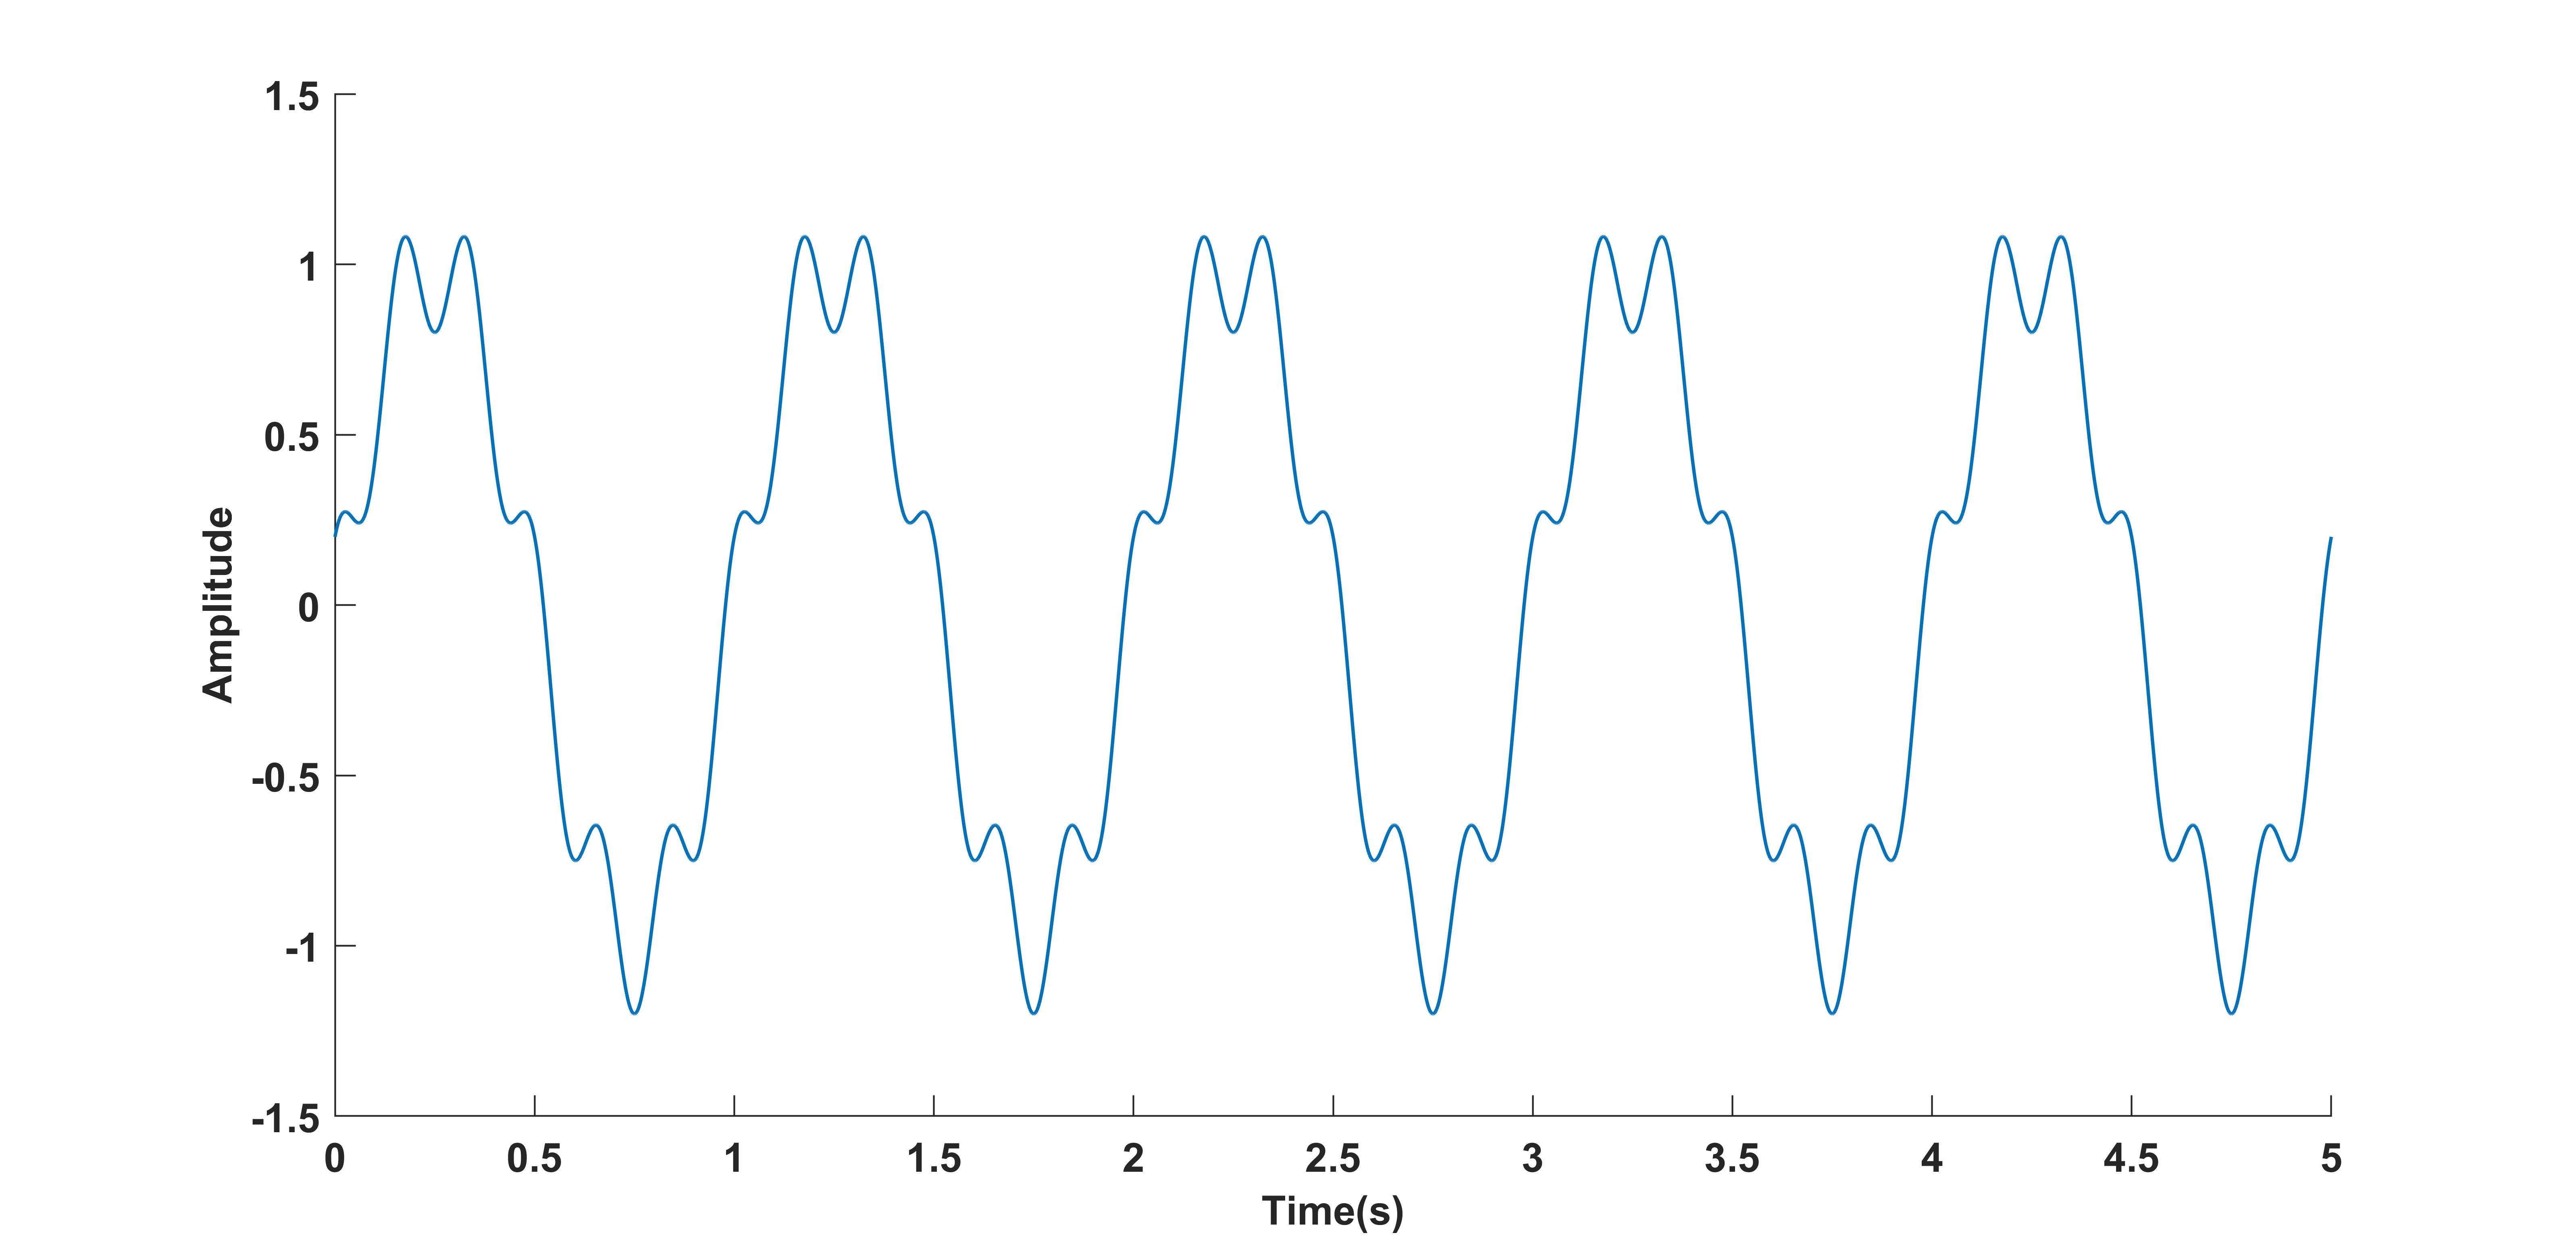
\includegraphics[width=5cm]{signal.jpg} \(\rightarrow\)
        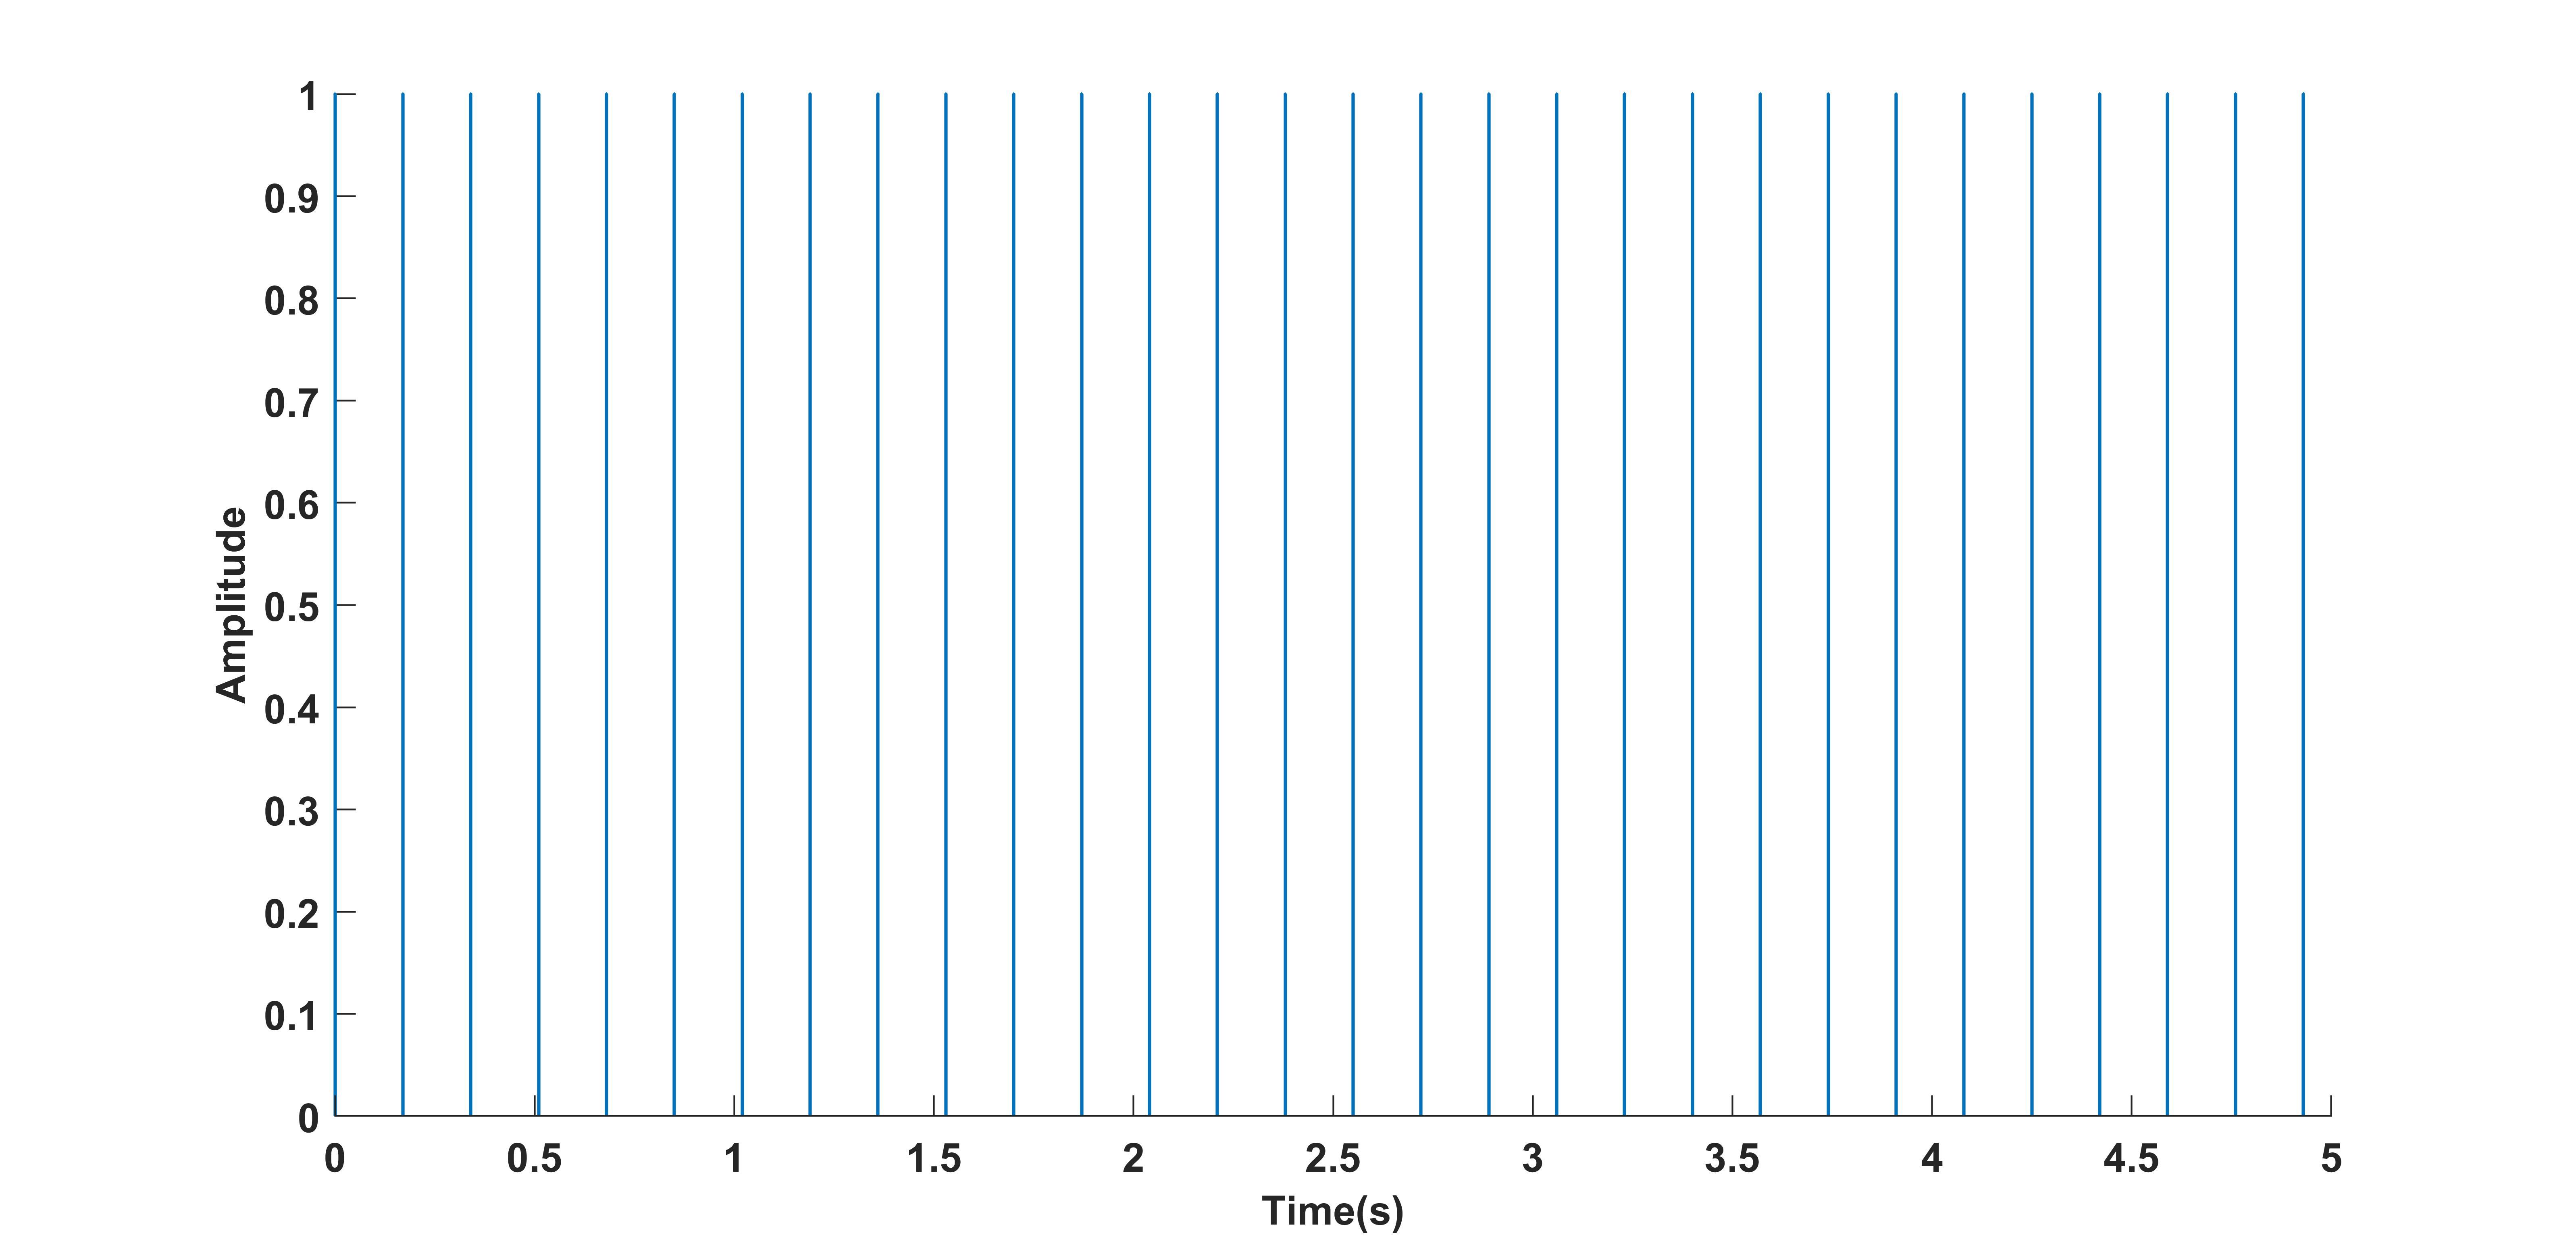
\includegraphics[width=5cm]{inpulse.jpg} \(\rightarrow\)
        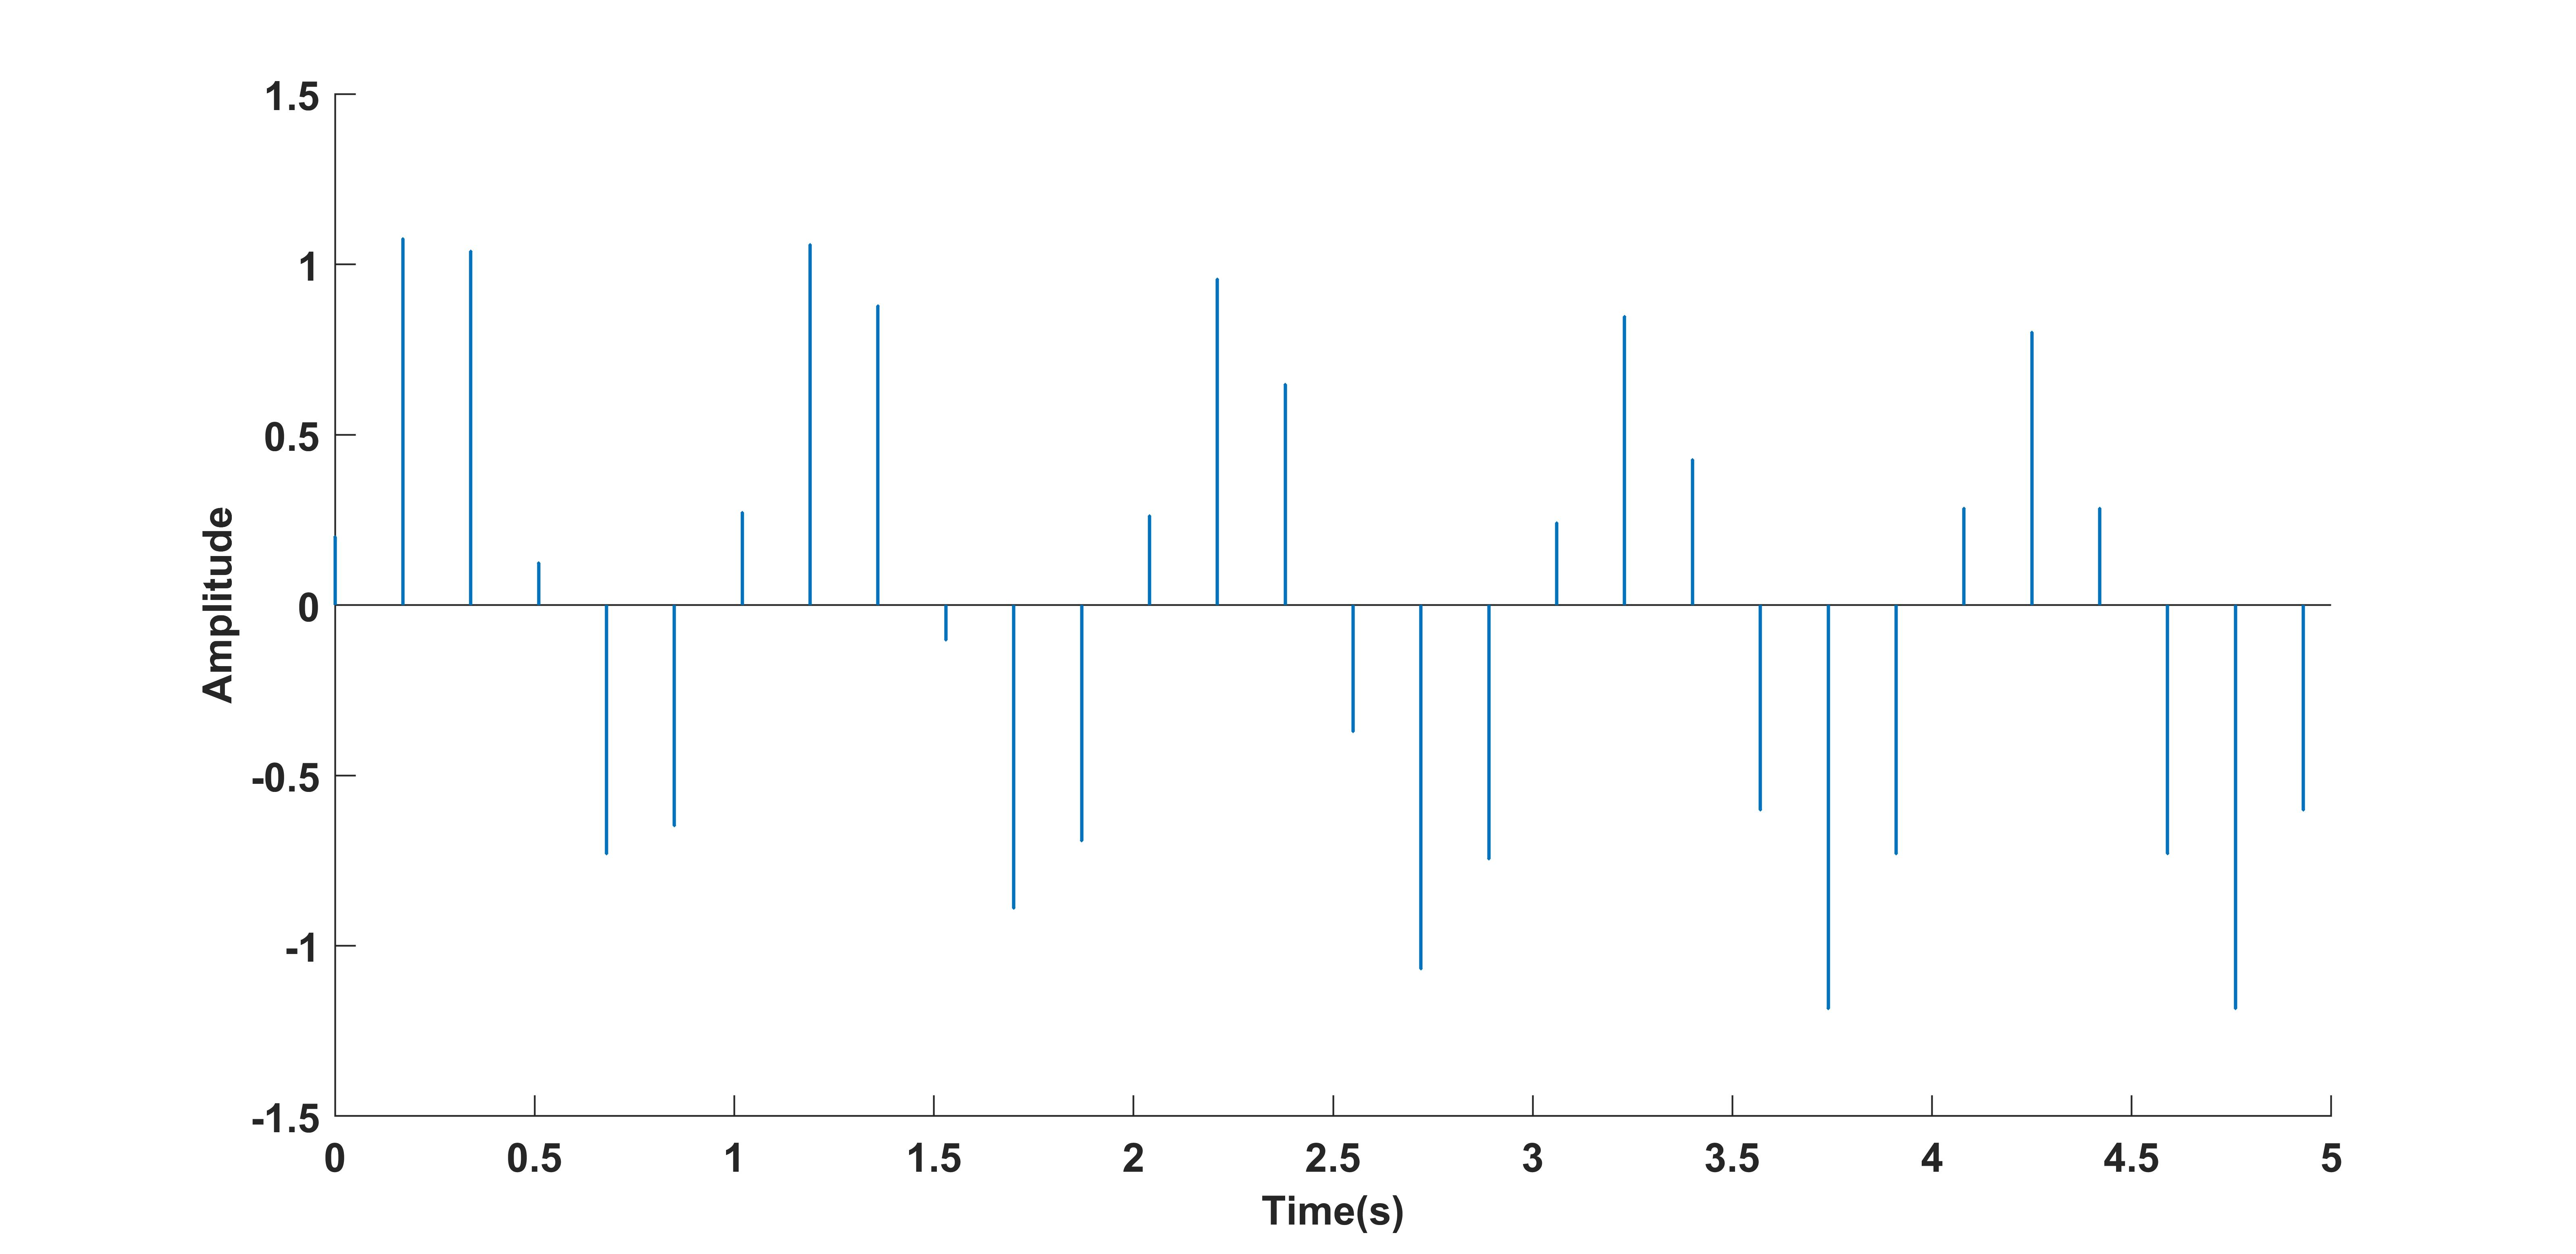
\includegraphics[width=5cm]{sampling_lias.jpg}
        \caption{Sampling illustration of a signal. From left to right Signal in continuous time domain,
        impulse input signal and sampled signal.}
\end{figure}
As show above, to get a discrete time signal  the input signal is multiply by an impulse of amplitude
1 shifted by kT with T the period and K the nth shifted of the impulse.\\
\begin{equation}
    f_s(t)=T\sum_{k=-\infty}^{\infty} f_i(kT)\delta(x-kT)
\end{equation}
One issue during sampling of signal come generally from the sampling period or frequency. In fact, the sampling 
frequency affects the signal during reconstruction. If the signal is sampled at period very high or slash with 
an impulse with high period, the discrete points output would be scattered with a pattern that will look nothing like
the input signal. Harry Nyquist, an electronic engineer, came up with a know maximum frequency at which a 
signal can be sampled to still represent the origin input signal as 

\begin{equation}
    \Omega_s > 2\Omega_{Niq}
\end{equation}
\(\Omega_{Niq}\) is known as the Nyquist frequency and \(\Omega_s \) the sampling frequency
\subsection*{Reconstruction}
The signal sampled above can be reconstructed into a continued signal perfectly but there is a catch. Shannon 
theory stated that to be able to reconstruct a signal, one must not only sampled the input at \(\Omega_s > 2\Omega_{Niq}\)
but also passed it through an ideal low pass filter. From the above section we known what Nyquist principle is 
, thus let see what an ideal low pass filter is.\\
\begin{itemize}
    \item Perfect Ideal Low Pass Filter \\
    An ideal low pass filter (ILP) has the following form\\
    \begin{equation}
        H(\Omega)=\{T_s; -f_{c}<t<f_c
    \end{equation}
    and zero everywhere else as shown in the figure bellow.
    \begin{figure}[h]
        \centering
            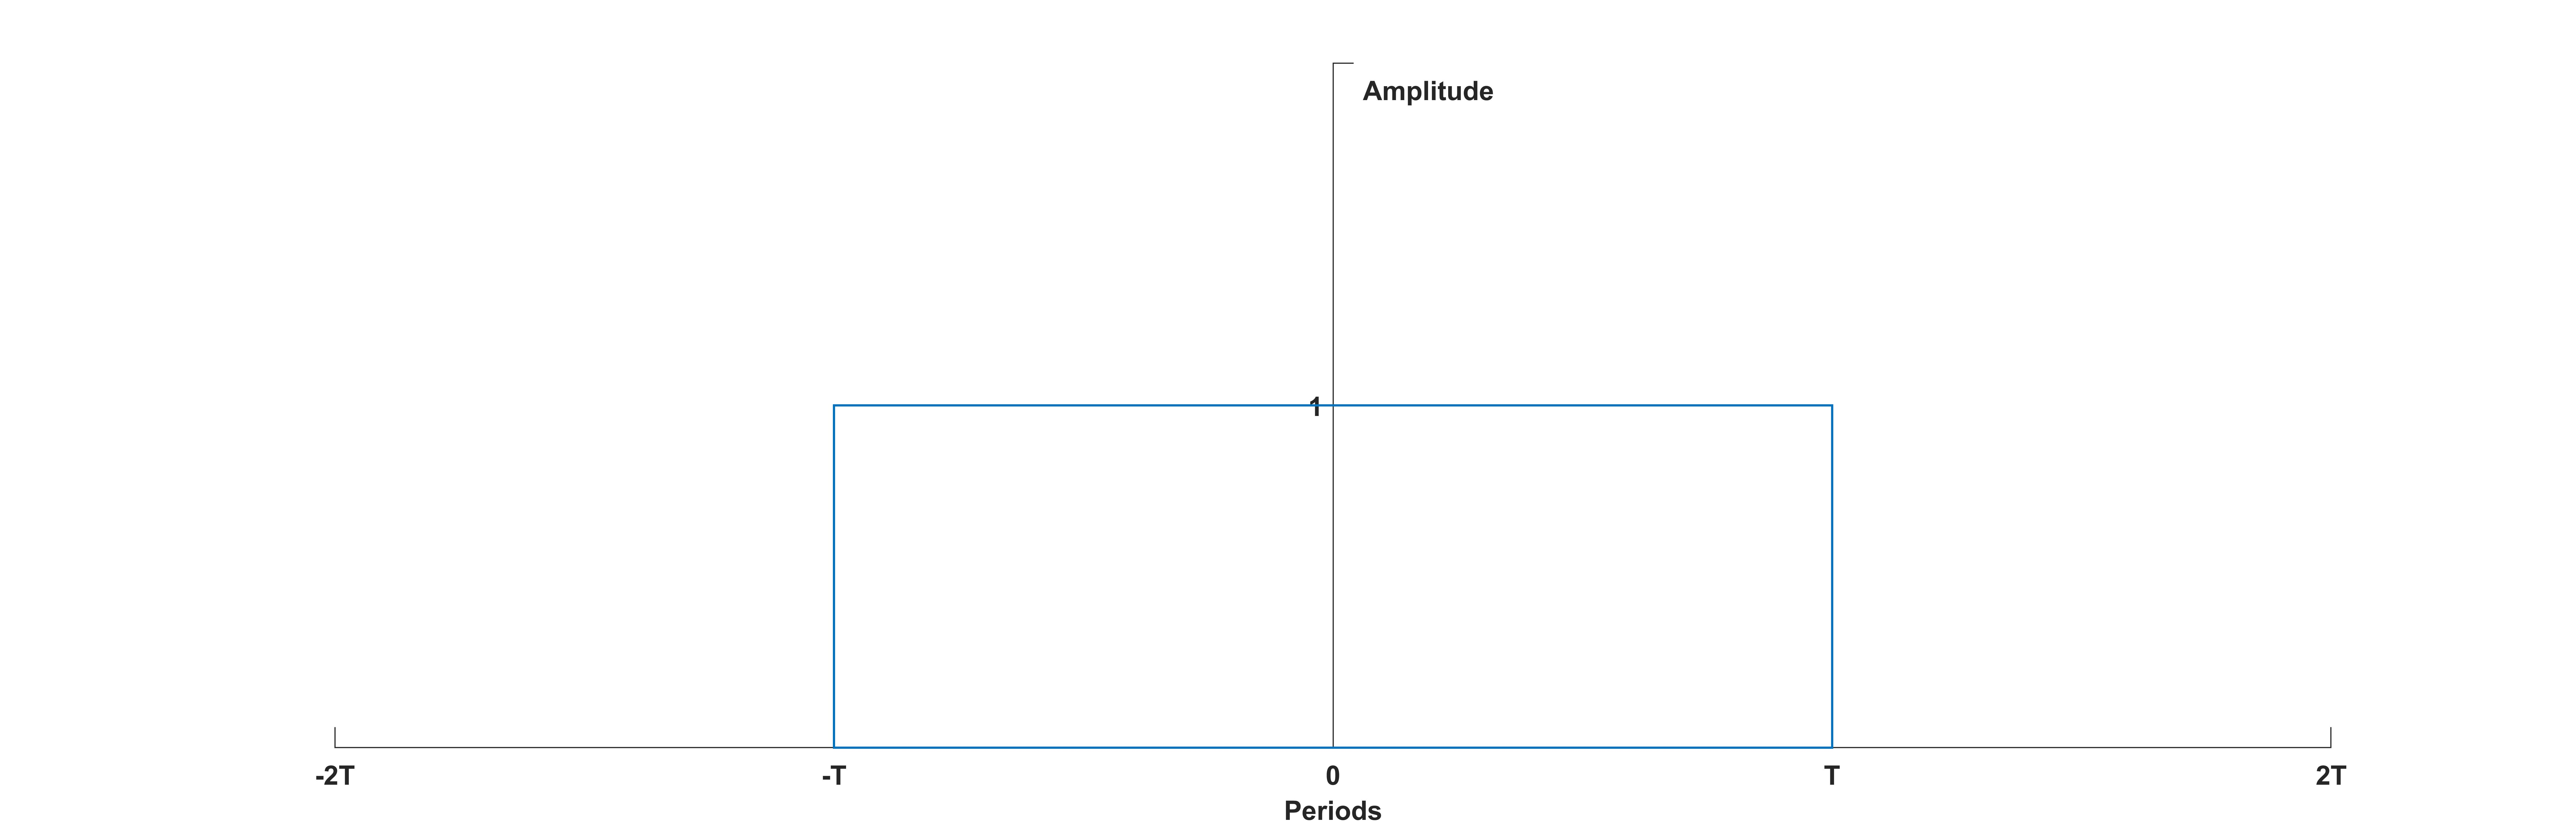
\includegraphics[width=15cm]{Lowpass.jpg}
            \caption{An ideal LP filter with amplitude 1 and cut-off frequency of \(f_c\)}
    \end{figure}
    The impulse response response of such signal can be found using
    \begin{equation}
        h(t)=\int_{-f_{c}}^{f_c}e^{-j\Omega t}d\Omega
    \end{equation}
    after performing the integration, the above function become 
    \begin{equation}
        h(t)=\frac{sinc(f_{c}t)}{f_{c}t} 
    \end{equation}
    the sinc function can be plotted in MatLab to obtain the figure bellow.
    \begin{figure}[h]
        \centering
            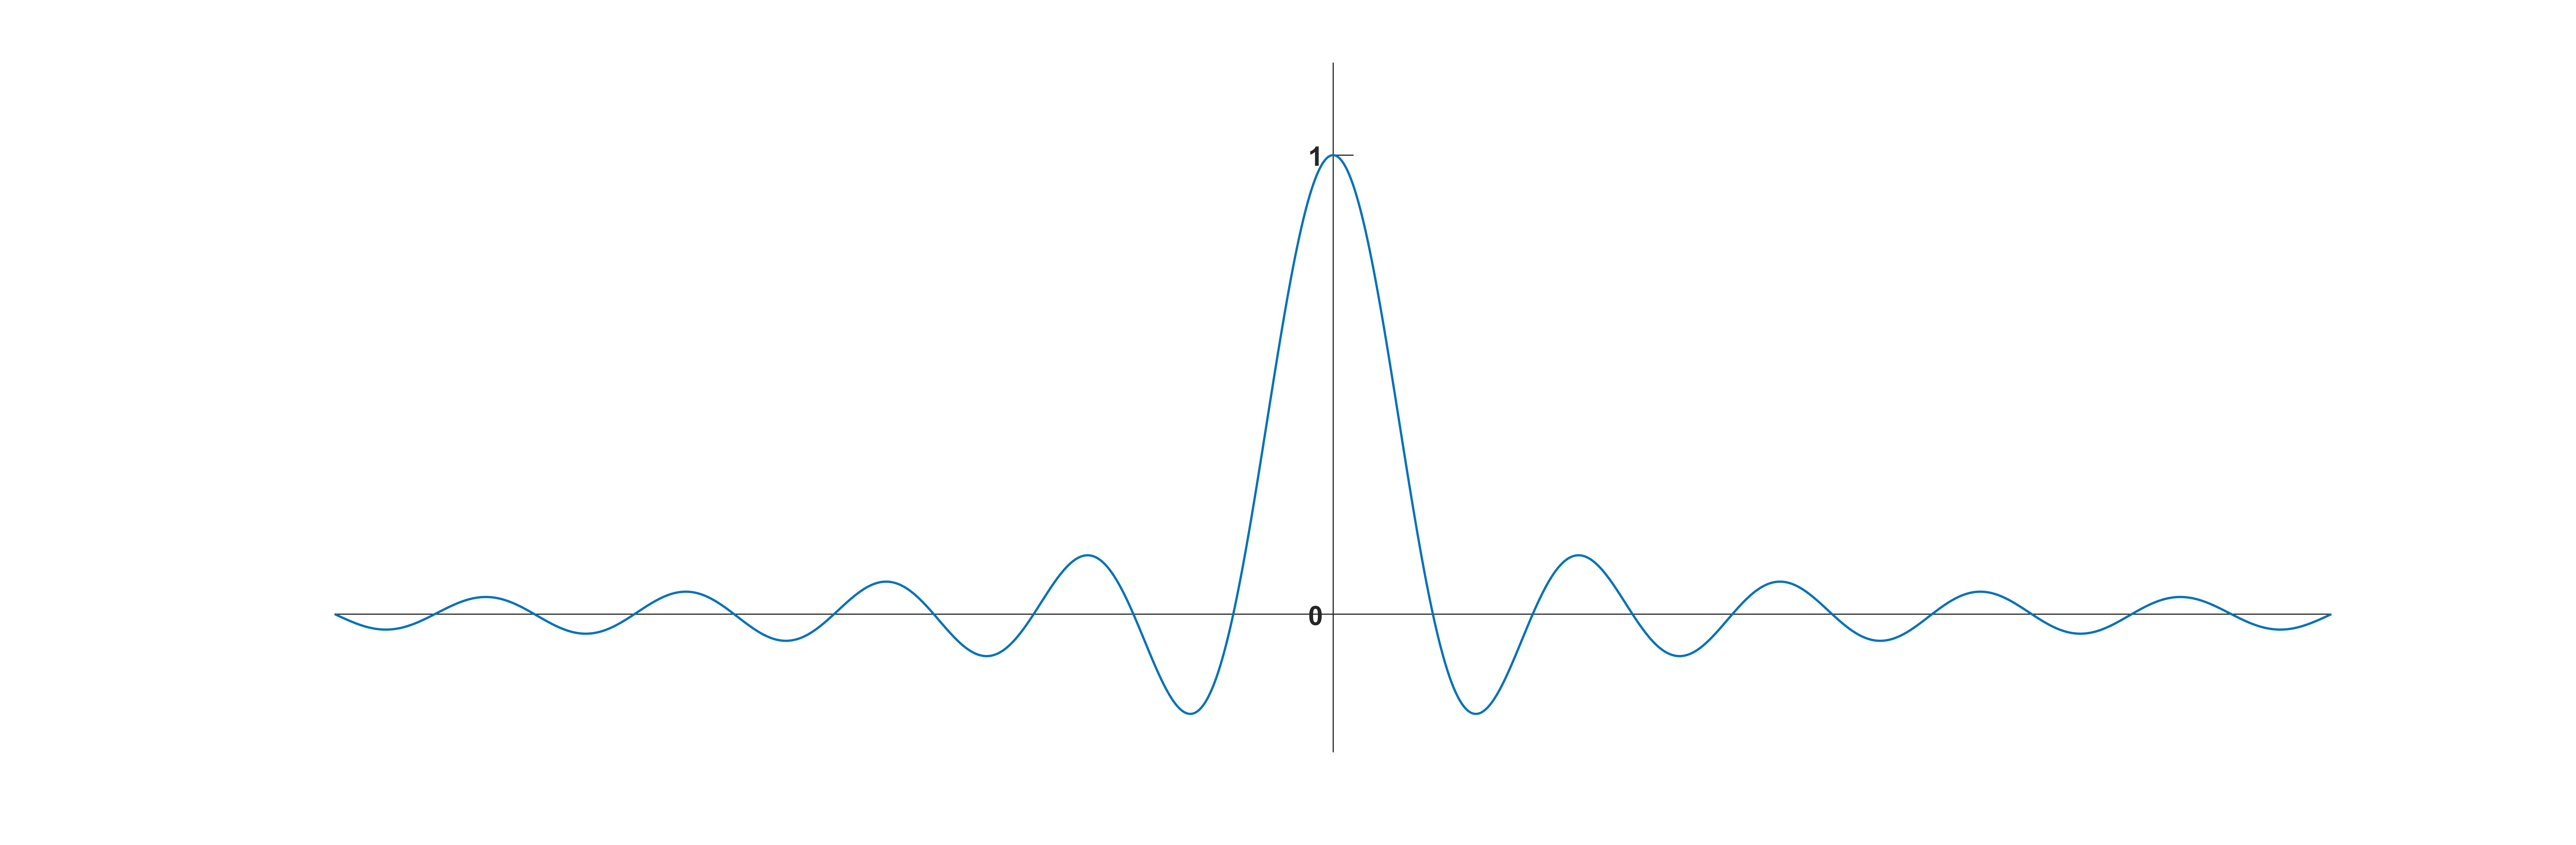
\includegraphics[width=15cm]{sinc.jpg}
            \caption{plot of the sinc function derive from the above low pass filter}
    \end{figure}
    It can be seen from the figure that, the continuous time signal of a ILP is not causal. In fact, the system
    responded before even it has bee kicked, in other word before time started as we can not consider negative time.
    This sort of system is not real and can not be implemented in real life. Thus, Shannon theory can not be used 
    in real system leading to the conclusion that a signal can not be perfectly reconstructed using real life
    hardwares with this sort of low-pass filter. Nonetheless, we can reconstruct the signal
    perfectly using MatLab provided that the sampling frequency respect the Nyquist rule.\\
    When sampling at the period of 0.017
    \begin{figure}[h]
        \centering
            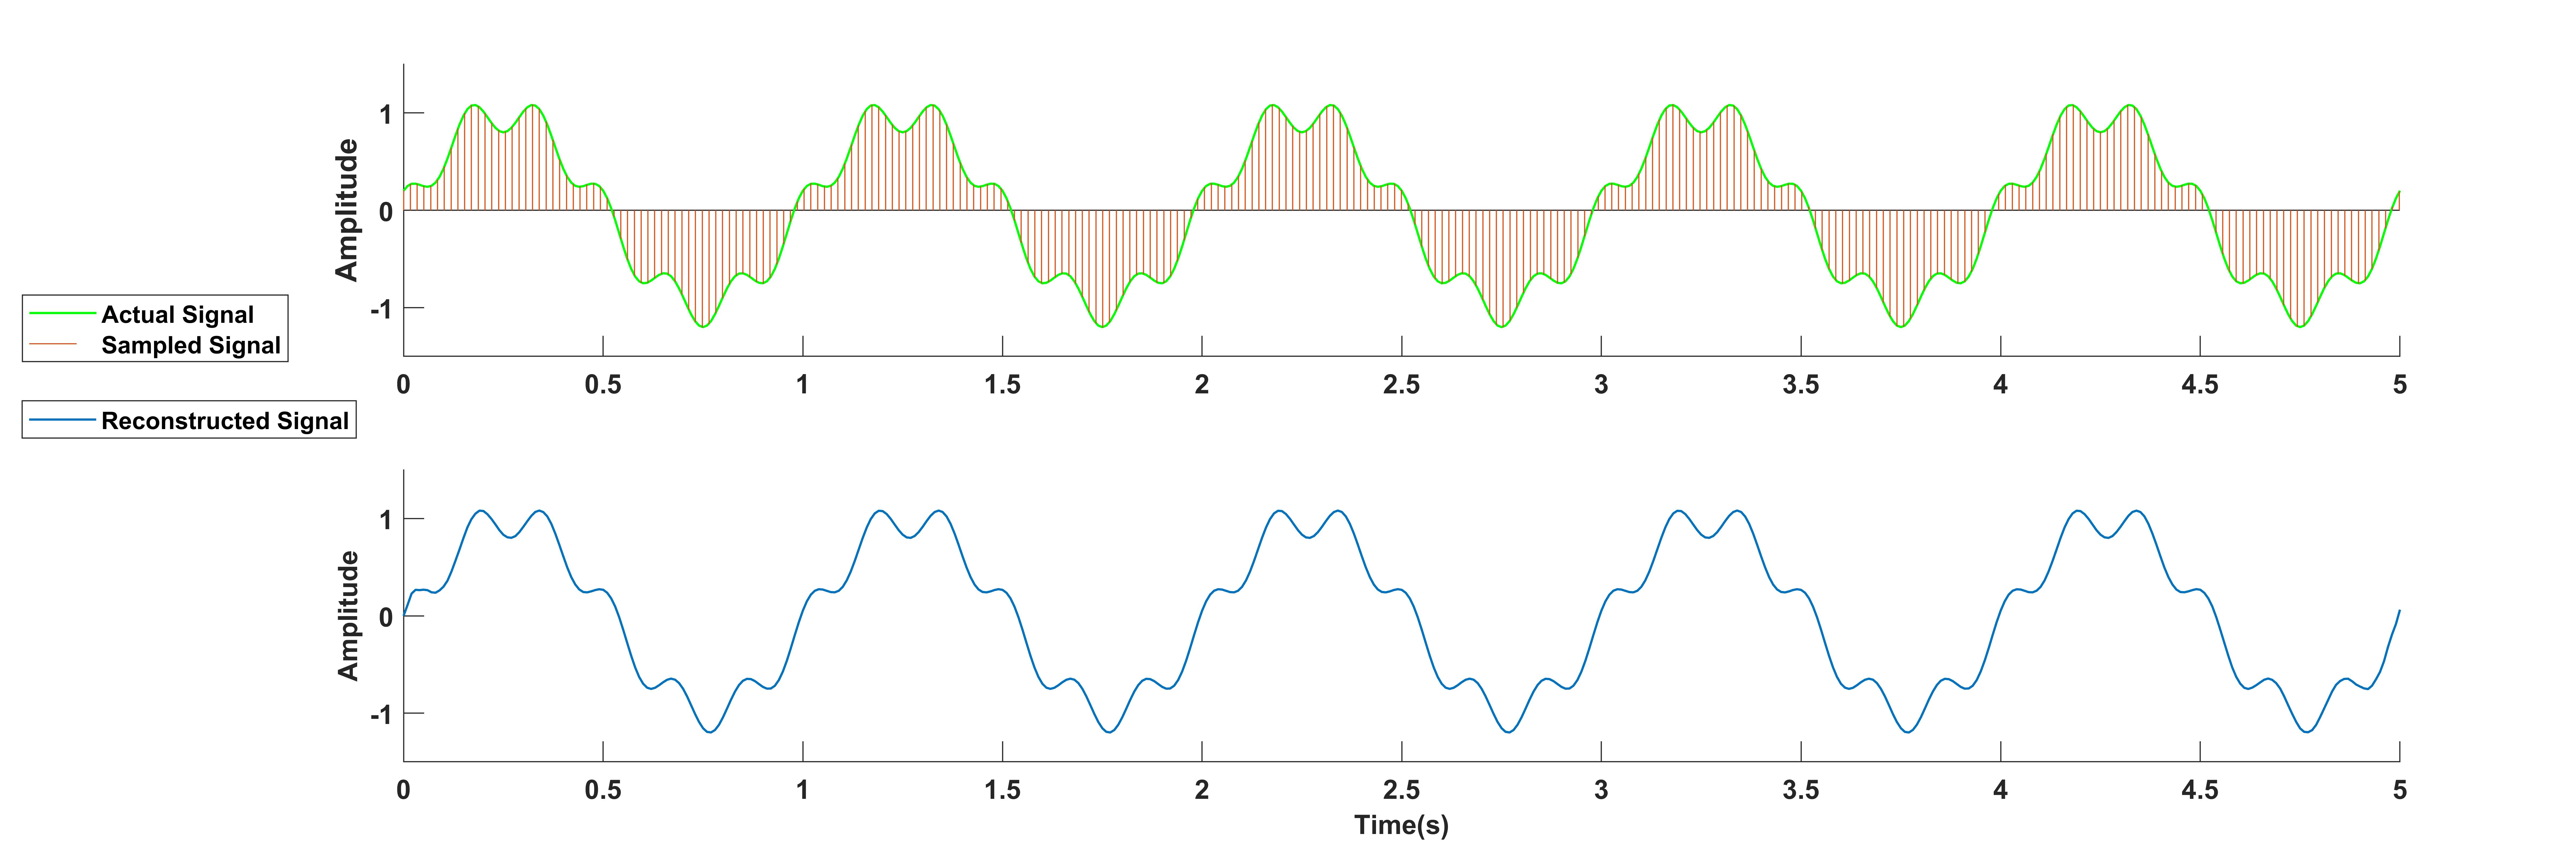
\includegraphics[width=15cm]{Reconstructed_0017.jpg}
            \caption{Reconstructed signal sampled at T=0.017s. The top figure
            is the sampled signal and bottom represent the reconstructed Signal
            using Matlab and the sinc function}
    \end{figure}
    The signal can be reconstructed to match exactly the analog input
    but the if the signal is sampled at a period ten times slower, it become obvious that
    \begin{figure}[h]
        \centering
            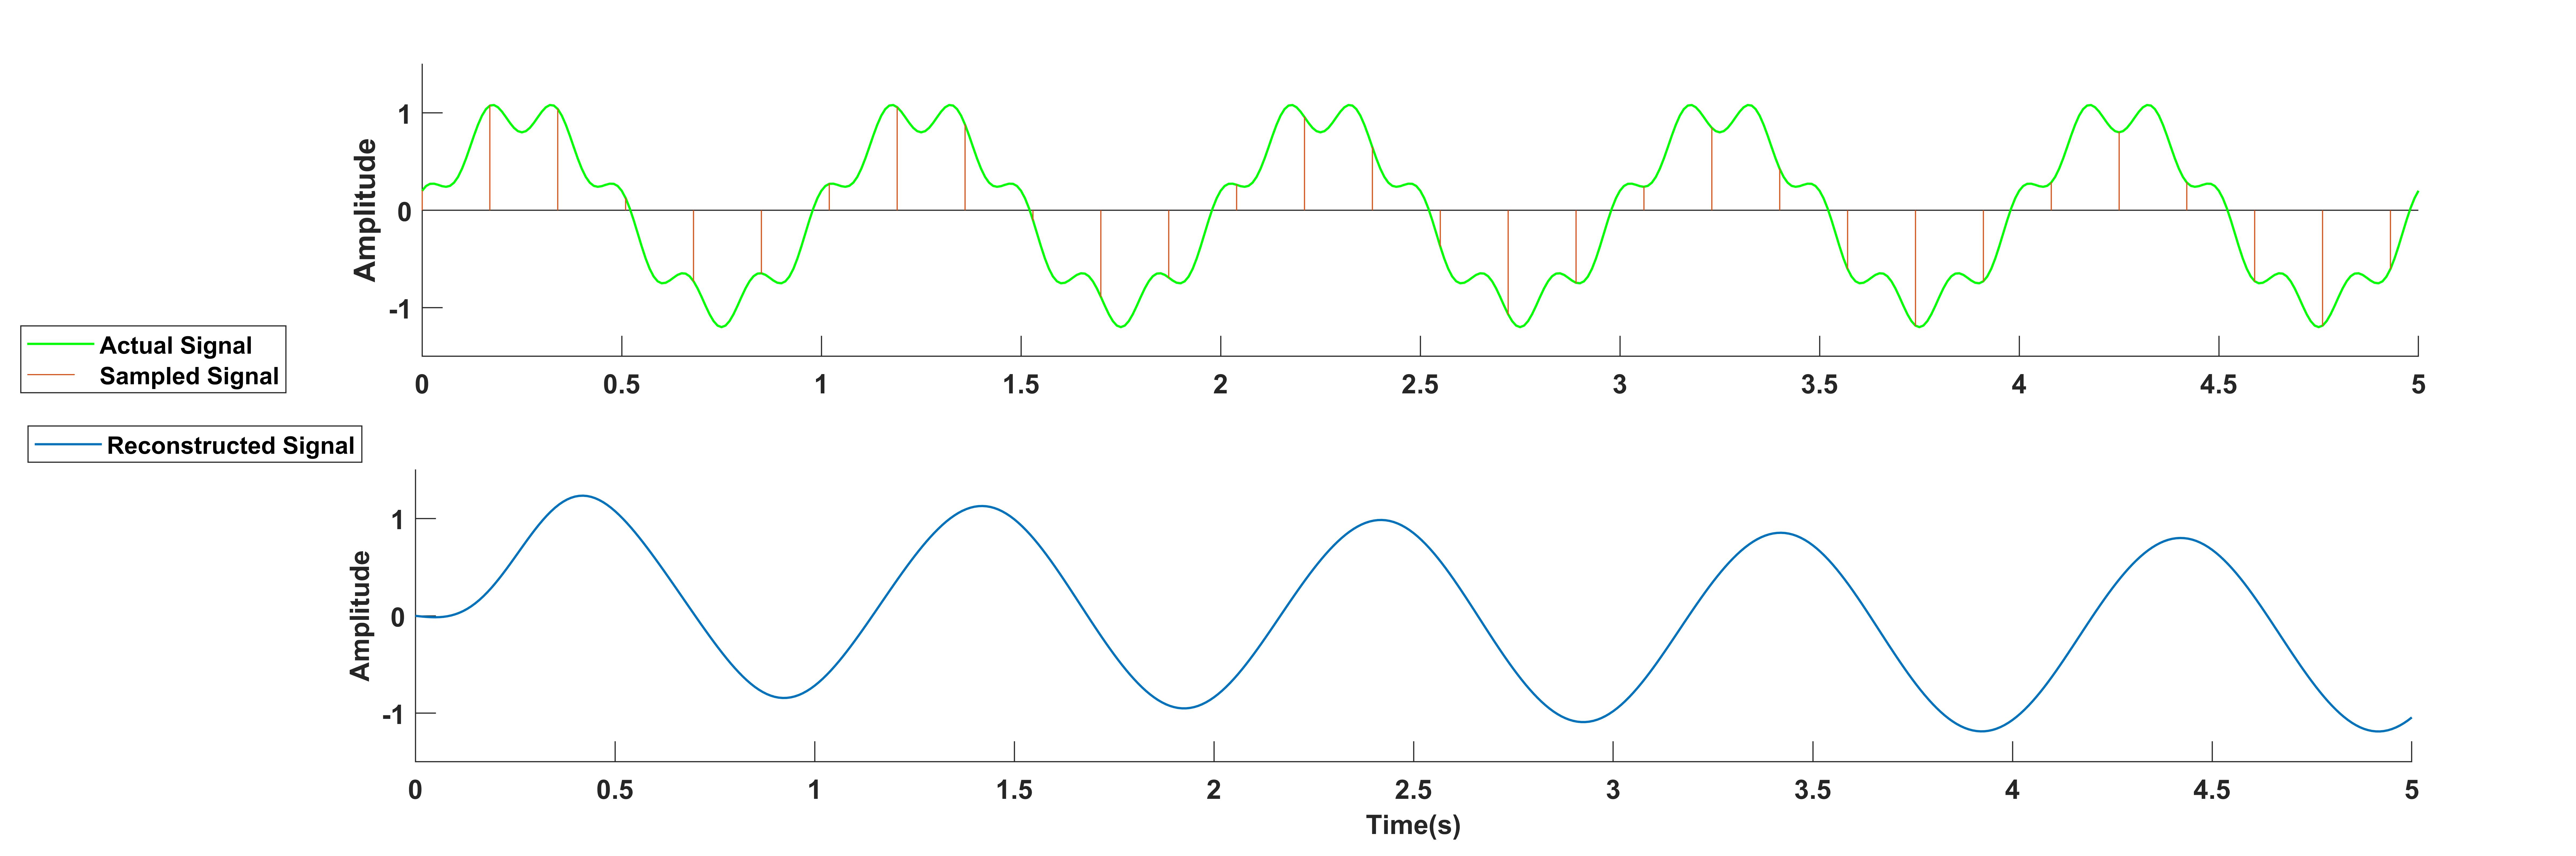
\includegraphics[width=15cm]{Reconstructed_017.jpg}
            \caption{Reconstructed signal sampled at T=0.17s. The top figure
            is the sampled signal and bottom represent the reconstructed Signal
            using Matlab and the sinc function. The reconstructed signal is liaised}    
        \end{figure}
    the reconstructed signal does look nothing like the input signal. This phenomena is know as 
    liaising. 
    As mentioned above, a perfect low pass filter can not be design 
    in real life, thus engineers have come with many brilliant ideas
    to design ADC and DAC. 
    \item Zero Order Hold (ZOH)
    Zero oder hold consist of using the nth value of the sampling signal
    and hold it until the next value is available. Any signal can then be reconstructed
    closed to accuracy using this method if the sampled period is small
    enough. Mathematically it can be showed that the amplitude of the frequency 
    response of ZOH is 
    \begin{equation}
        \mid G_{ZOH}(j\omega)\mid =T\mid \frac{sin(\omega T/2)}{\omega T/2}\mid
    \end{equation}
    and the phase shifted is 
    \begin{equation}
        \phase {G_{ZOH}(j\omega)} =\frac{\omega T}{2} + \phase{sin(\omega T/2)}
    \end{equation}
    The bode plot of the ZOH is as follow
    \begin{figure}[h]
        \centering
            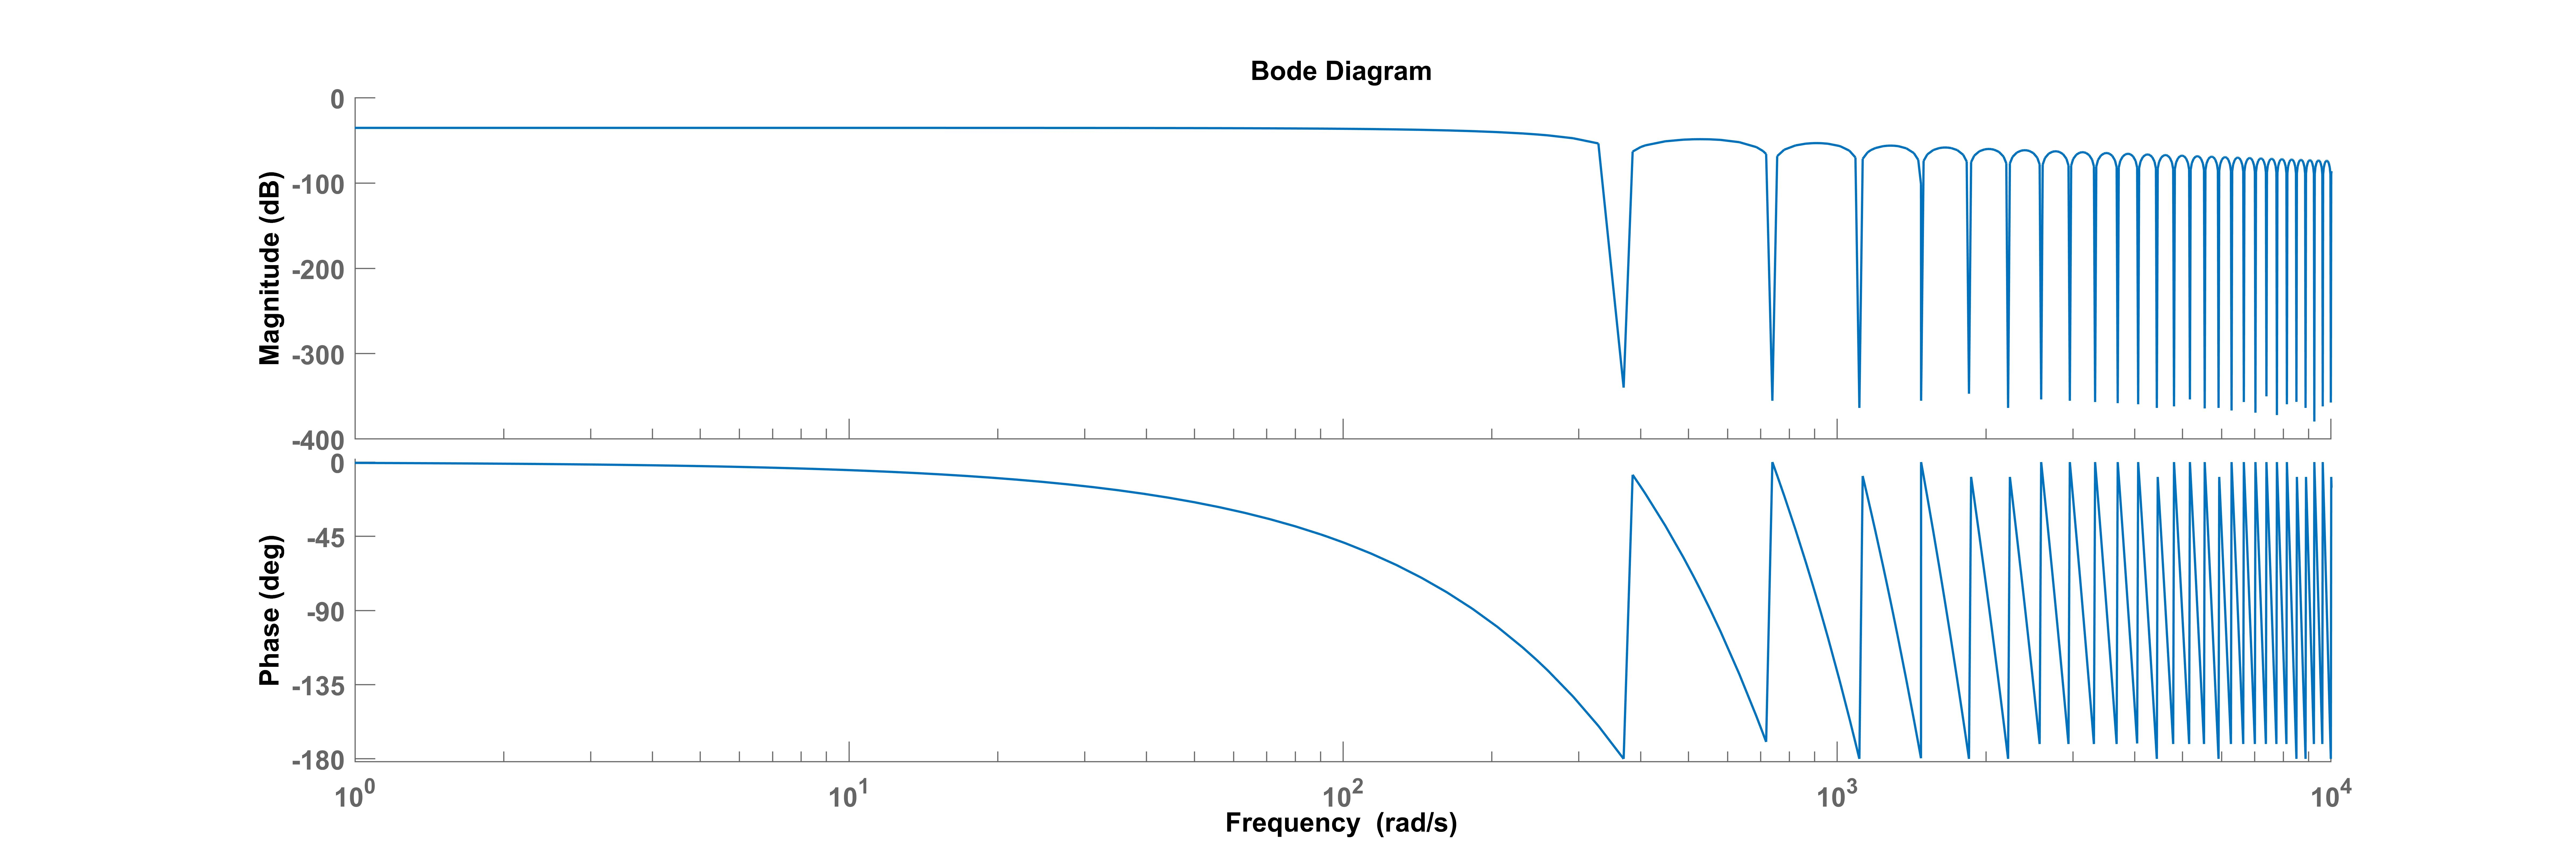
\includegraphics[width=15cm]{bode_ZOH.jpg}
            \caption{Bode plot of Zero oder hold. The phase shift
            of the system is zero for frequency lower than 100 rad/s}
    \end{figure}
    Using MatLab, the signal can also be reconstructed using the ZOH. For each value
    of the sampled signal, and array of known size can be created and 
    populated with each data point. Doing so for all elements of the sampled
    data points Matlab will generate an array which plotted should 
    look like the one bellow. 
    \begin{figure}[h]
        \centering
            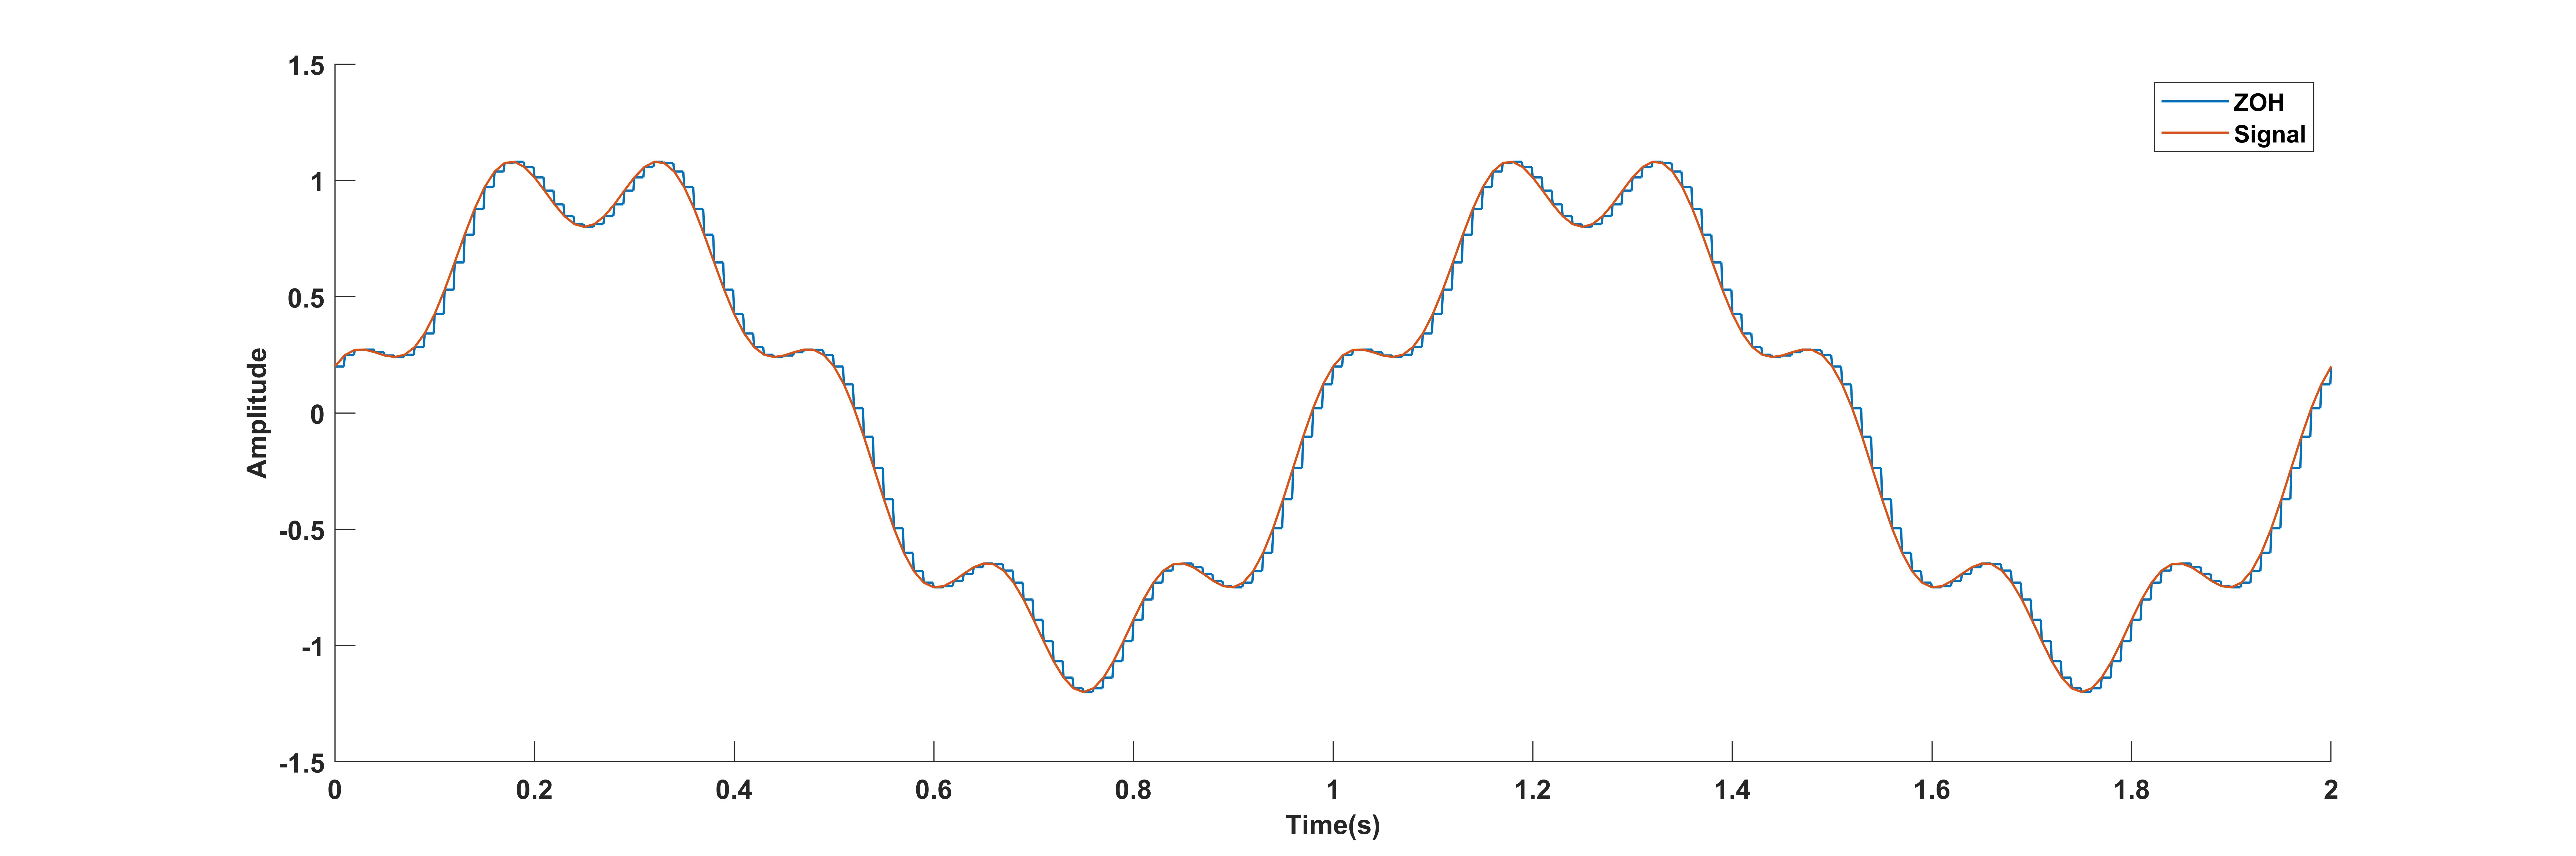
\includegraphics[width=15cm]{ZOH.jpg}
            \caption{Zero order hold low pass filter, the resolution of the 
            reconstructed in dependent of the sampling period}
    \end{figure}
    As it can be seen on the above plot, the accuracy of the ZOH depend 
    on the sampling period of the Signal
    \item Acausal First Order Hold(AFOH)\\
    AFOH uses interpolation to Predict the next value of the signal. When reconstructing using
    AFOH, the n-1 and n are used to found a value in between. Depending of 
    the sampling  period, the reconstructed signal has higher resolution
    than the ZOH. In fact, 2x point is generated with period of Ts/2. 
    \begin{figure}[h]
        \centering
            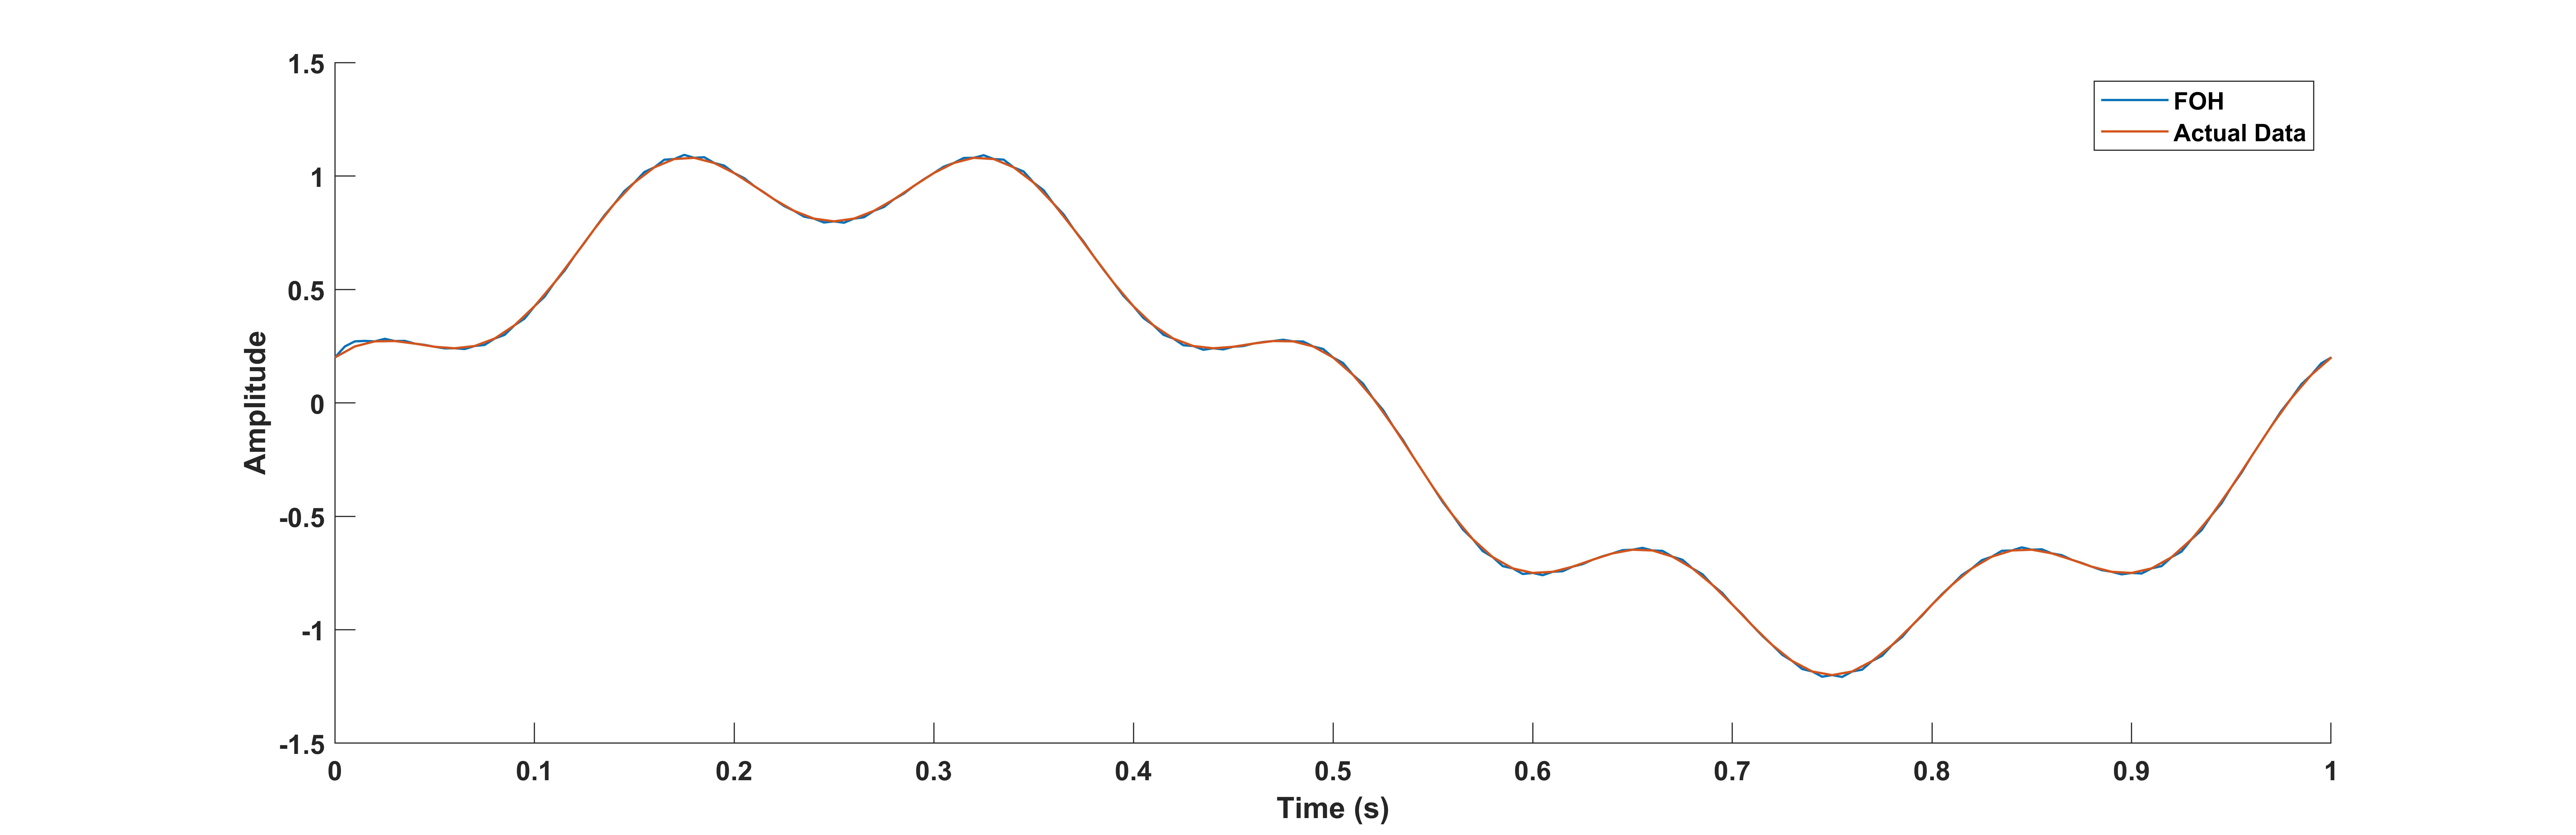
\includegraphics[width=15cm]{FOH_2_p.jpg}
            \caption{Acausal first order hold signal reconstructed using Matlab. The reconstruction
            uses interpolation method}
    \end{figure}
    The above figure show the AFOH using matlab. The code can be found attached to
    this report.\\
    Mathematically, if the sampling signal of AFOH is 
    \begin{equation}
        x_s(t) =T\sum_{n=-\infty}^{\infty} \delta (t-nT)
    \end{equation}
    Then the laplace domain response of the signal is to be
    \begin{equation}
        H(s)=(\frac{1-e^{-sT}}{sT})^2
    \end{equation}  
    This type of system is realizable by designing a digital filter of gain  
    \(H(z) = 1-z^{-1}\) 
    The bode plot of the laplace domain transferer function is similar to the ZOH except 
    at high frequency
    \begin{figure}[h]
        \centering
            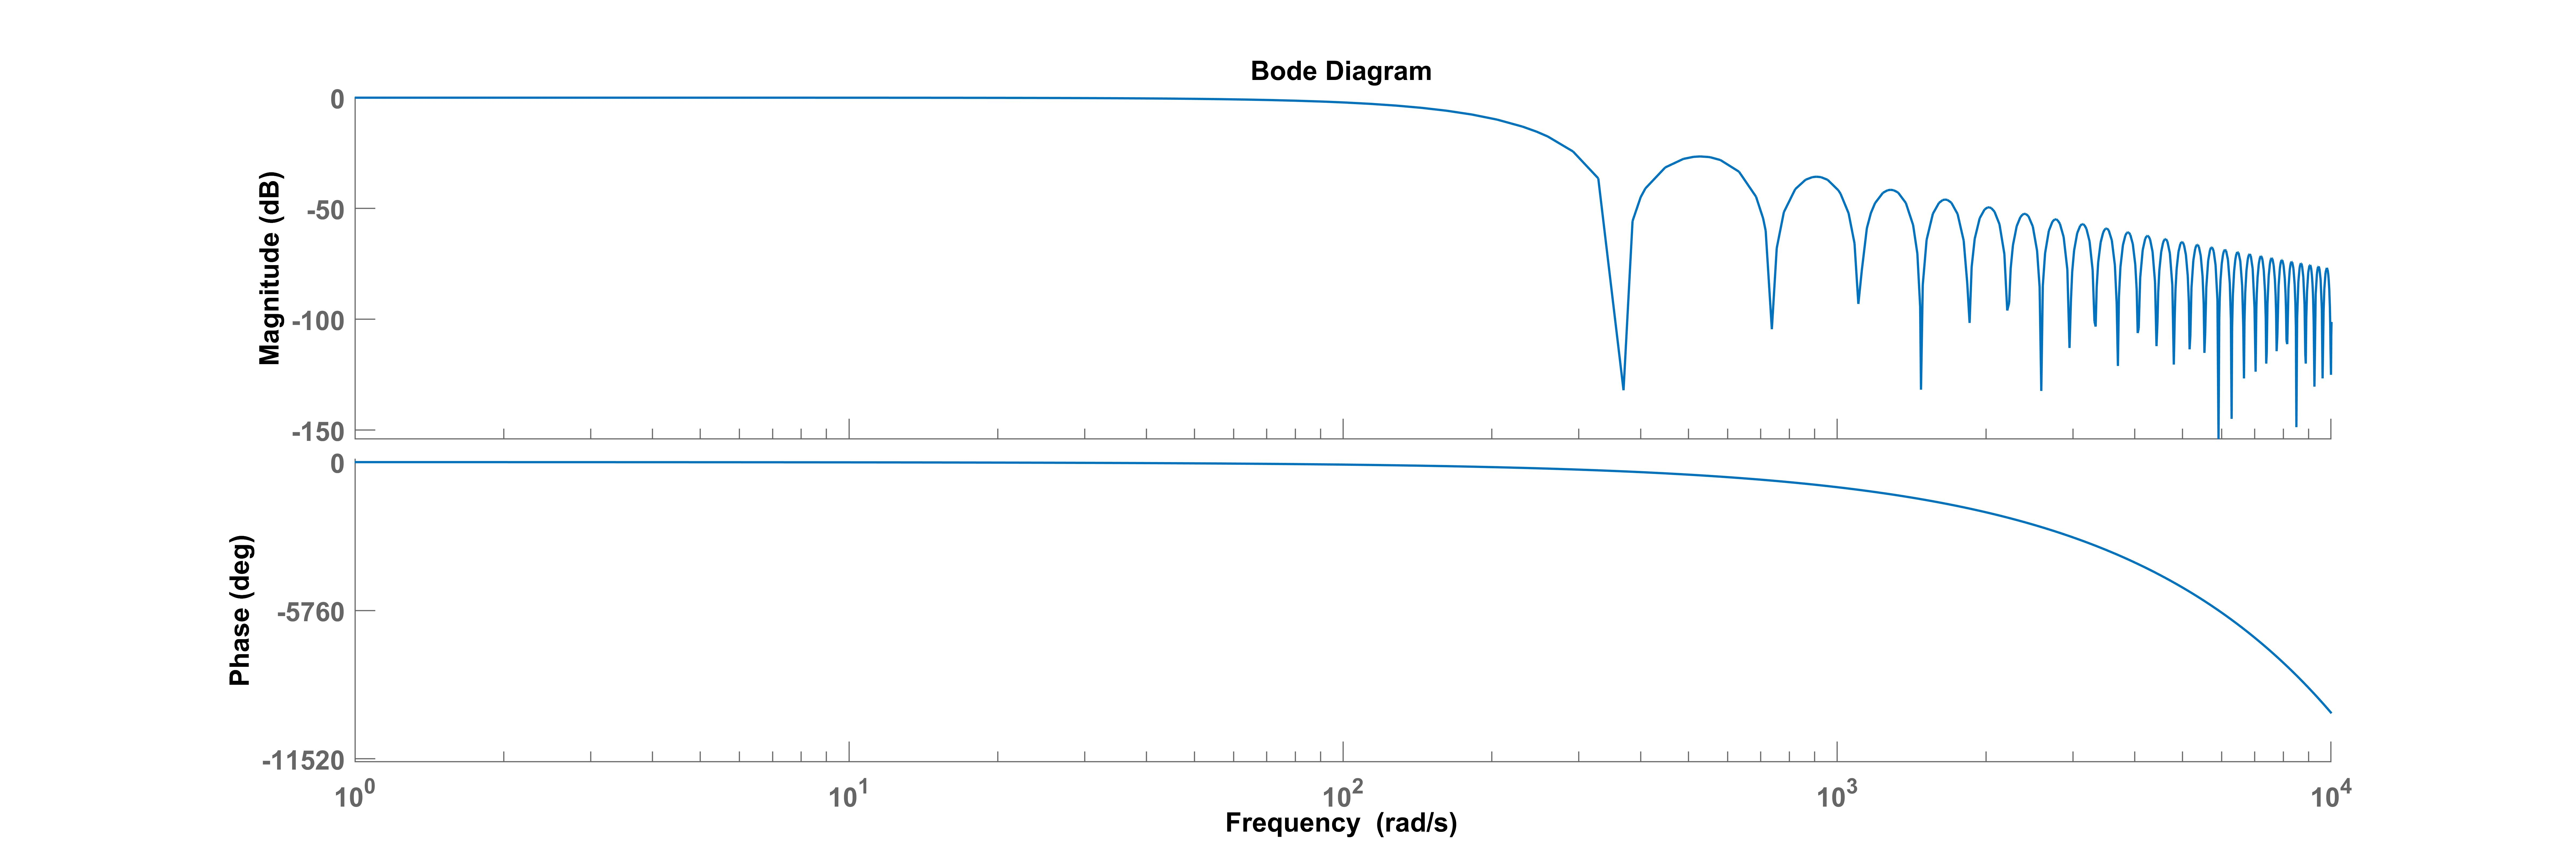
\includegraphics[width=15cm]{bode_FOH.jpg}
            \caption{Bode plot of First oder hold. The phase shift
            of the system is zero for frequency lower than 100 rad/s}
    \end{figure}
    \item Predictive First Order Hold (PFOH)
    Unlike  AFOH, PFOH uses extrapolation. The knowing the values of the
    n-2 and n-2 data point, extrapolation is used to get a value of the n position before 
    such data point is collected. 
    \begin{figure}[h]
        \centering
            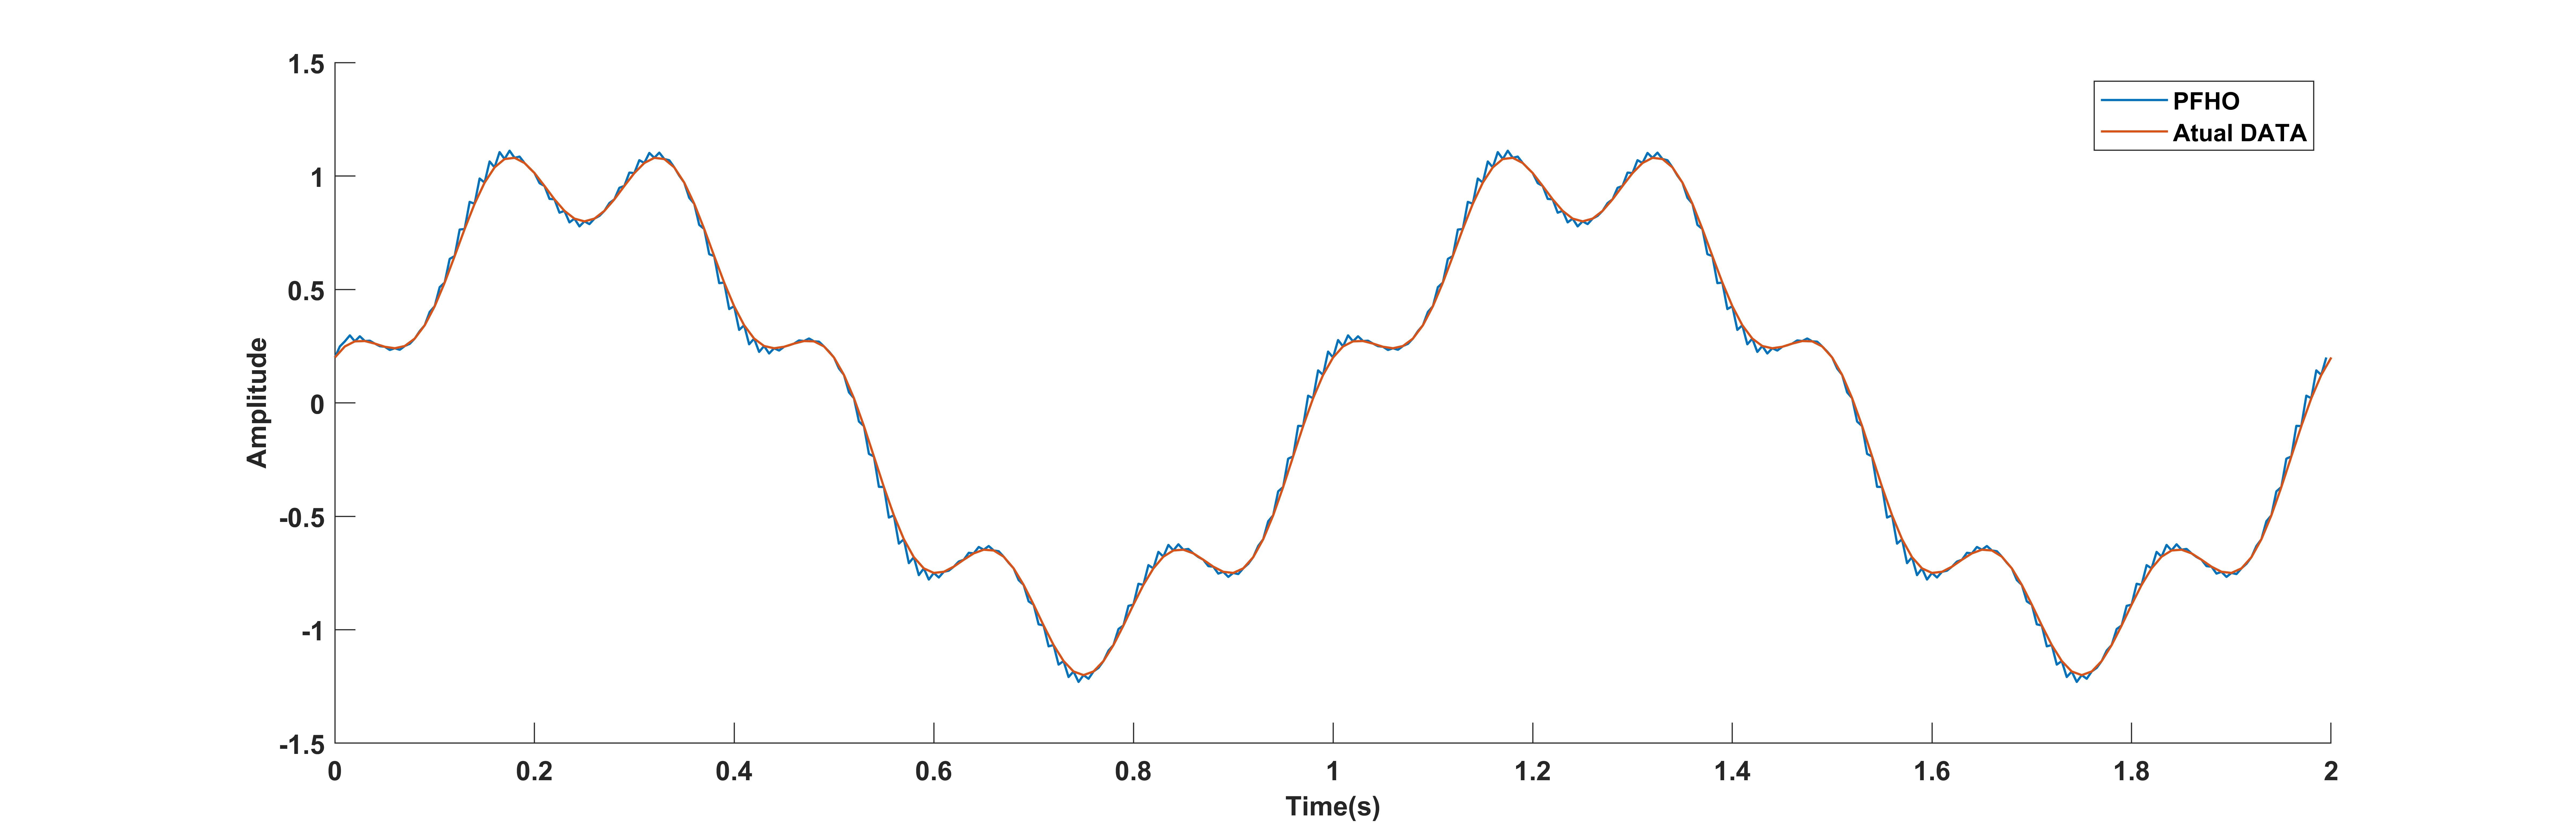
\includegraphics[width=15cm]{PFOH.jpg}
            \caption{Reconstructed signal of predicted first order hold using extrapolation}
    \end{figure}
    PFOH  has lower resolution than the AFOH. This can be seen on the figures 7 and 8
    Both system can be design in real life by creating filter that 
    mimic the same principles. 
    \begin{equation}
        H(s)=(1+sT)(\frac{1-e^{-sT}}{sT})^2
    \end{equation}
    The laplace domain equation of a PFOH is shown above. The main different is that
    PFOH has an extra zero which could make the system complex to design
\end{itemize}
\section*{Conclusion}
Any signal can be reconstructed using a giving filter. In the perfect world, an ideal low pass
filter can be used to reconstruct any signal perfectly if it is sampled
following the Nyquist principle (Shannon theorem). Though such system
is impossible to design, other technics such as ZOH, AFOH and PFOH 
are great tools to reconstruct signal with create accuracy. ZOH is the less
accurate but easy to implement. In the other hand AFOH has a greater accuracy and can be easy to design. However, AFOH shift the 
reconstructed signal due to delay.
\appendix
\begin{thebibliography}{9}
\bibitem{wikipadia} 
"First-order Hold." Wikipedia. January 02, 2019. Accessed March 14, 2019. 
\bibitem{Book} 
"Digital Control of Physical system", Chapter 2, page 1-14.
\bibitem{Overleaf} 
"Documentation." Overleaf, Online LaTeX Editor. Accessed March 14, 2019. https://www.overleaf.com/learn/latex/.
\end{thebibliography}
\lstset{language=Matlab,%
    %basicstyle=\color{red},
    breaklines=true,%
    morekeywords={matlab2tikz},
    keywordstyle=\color{blue},%
    morekeywords=[2]{1}, keywordstyle=[2]{\color{black}},
    identifierstyle=\color{black},%
    stringstyle=\color{mylilas},
    commentstyle=\color{mygreen},%
    showstringspaces=false,%without this there will be a symbol in the places where there is a space
    numbers=left,%
    numberstyle={\tiny \color{black}},% size of the numbers
    numbersep=9pt, % this defines how far the numbers are from the text
    emph=[1]{for,end,break,if},emphstyle=[1]\color{red}, %some words to emphasis
    %emph=[2]{word1,word2}, emphstyle=[2]{style},    
}

\section*{Matlab Code}

\lstinputlisting{project_3.m}
\end{document}
